\documentclass[a4paper, 12pt]{article}

\usepackage[utf8]{inputenc}
\usepackage{amsmath}
\usepackage{amsfonts}
\usepackage{amssymb}
\usepackage[a4paper]{geometry}
\usepackage{enumitem}
\usepackage{color}
\usepackage{hyperref}
\usepackage{booktabs}
\usepackage{float}
\usepackage{graphicx}
\usepackage{titlesec}
\usepackage{tcolorbox}
% \documentclass[tikz,border=5pt]{standalone}
\usepackage{pgfplots}
\pgfplotsset{compat=1.18}
\usepackage[backend=bibtex, style=numeric]{biblatex}
\addbibresource{thesis.bib}

\hypersetup{
	colorlinks=true, 
	linktoc=all,     
	linkcolor=blue,
	linktocpage
}

\titleformat{\section}[display]{\Large\bfseries\itshape}{}{0ex}
{\rule{\textwidth}{0.3pt}\vspace{0ex}
	\centering}[\vspace{-1ex}\rule{\textwidth}{0.3pt}]

\titleformat{\subsection}[display]{\large\itshape}{}{0ex}{}[]

\newcommand{\unnumberedsection}[1]{
	\newpage
	\phantomsection
	\addcontentsline{toc}{section}{#1}
	\section*{#1}}
\renewcommand\thesubsection{\Roman{subsection}}

\parindent0mm
\parskip1.5ex plus0.5ex minus0.5ex


%%% Title page
\title{\rule{\textwidth}{1.5pt}\vspace{0ex}
	Research Diary
\vspace{-1ex}\rule{\textwidth}{1.5pt}}
\author{Caio Simon}
% \date{Calender week 37, 2022}
% \today

\begin{document}
	
\maketitle

\newpage

\subsection{To-Do (short-term)}
\begin{itemize}
    \item Action masking
    \item Allow teams to see their place in standings + also their strength score next to other teams.
    \item (To think about at least) Instead of having a fixed player cohort, maybe I can use Deep Sets.
    \begin{itemize}
        \item Gemini gave the useful idea of building a player encoder that every player goes through. Then I take the mean or max as ``global context'' variable, which I append to the matrix.
    \end{itemize}
    \item Allow teams to sign players --- free agency
    \begin{itemize}
        \item Initially agents will be able to observe player ratings, to make the simulation easier.
        \item Must add preferences for players --- past success of a team and how much money they are offering.
    \end{itemize}
    \item Create trades for players
    \begin{itemize}
        \item Apparently this is hard to do; the combinatorial space is huge, so I will have to read more about how to do this.
    \end{itemize}
    \item $\checkmark$ Player evolution (easier)
    \item  $\checkmark$ Player retirement
    \item $\checkmark$ New players in the league
\end{itemize}


\subsection{To-Do (long-term)}
\begin{itemize}
    \item \texttt{PettingZoo} environment where agents can sign players in the off-season.
    \item \texttt{PettingZoo} environment where agents can trade players
    \item \texttt{PettingZoo} environment where agents draft young players.
    \item Calibration of parameters (veeery long-term)
    \item Survival analysis for ageing players.
\end{itemize}

\newpage

\section{Weakenesses}
\begin{itemize}
    \item Initial talent distribution
    \item Parameters are guesstimated
    \item Game simulation is too basic
    \item Better players should account for a larger portion than end-of-bench players.
\end{itemize}

\section{Chronological Order}

\subsection{July 4, 2026}

I have been thinking about the issue of measuring tanking a bit more and I think I have a much better idea of what I want to do. This all goes back to that initial experiment I did, with distributing players randomly to teams and then having them play against each other. I'll put the image back here again.

\begin{figure}[h]
    \centering
    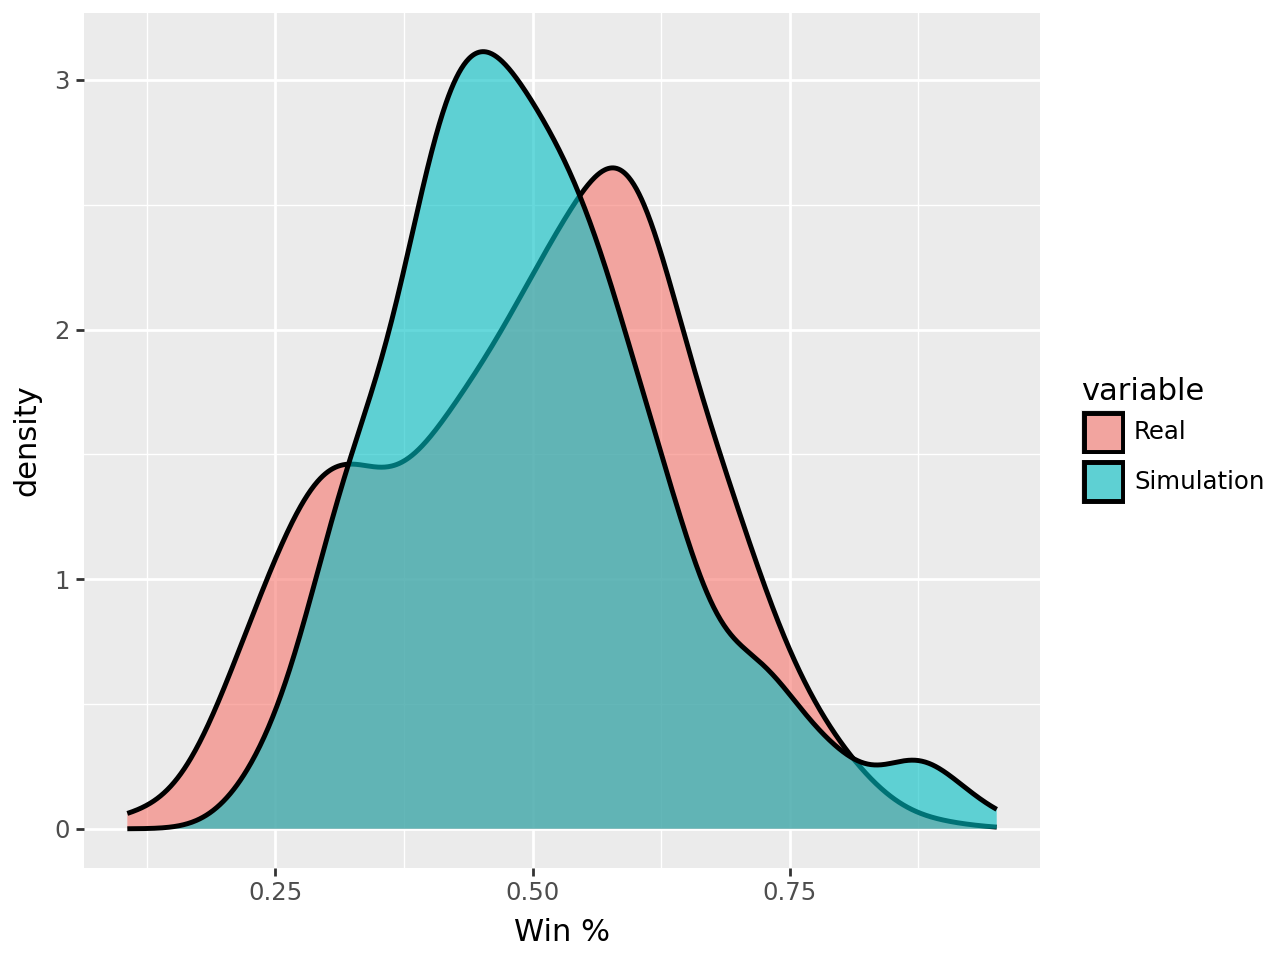
\includegraphics[width=0.75\textwidth]{figs/win_pct_plot.png}
    \caption{First look at simulated vs real win percentage. I don't get the slightly bimodal distribution yet, but I hope this will happen once teams start to make choices.}
\end{figure}

Before I was too myopic. I was looking only at trying to discern whether specific teams were tanking, but I don't care that much about micro behaviour in this project. Instead, I should be able to see the pattern at a macro level. By plotting the distribution of win percentages across different league rules, I can assess how bi-modal the distributions appear to be (a sign of tanking), and I can also compare distributions with metrics, like Wasserstein distance or KL divergence, to see how close they are to some idea distribution.

So for example, let's say I have an environment with no lottery. Teams are either randomly allocated young talent or they simply enter free agency. Then I train an agent whose only concern is to win a championship \footnote{I could also play with the discount rate, if need be}. Then I would have a ``win-maximising'' league, where no handouts are given, and teams have to make do with wily moves \footnote{I haven't thought about it yet, but I could also imagine having teams in this league still have some heterogeneity in how much they care about championships vs regular season win percentage and such}. The point is that I get league where there is no reward for losing. That is, unless you cut players for cap space (even then in order to win shortly after).

So then I gather many seasons of this type of league and I have a win percentage plot. I expect it to be some sort of normal distribution, probably slightly skewed towards the top end. I also gather data on my alternative leagues: the one with the current lottery, COLA, Nate Silver's Arcs, the old lottery system, the new proposed system, and so on. I would expect these leagues to have some form of bi-modality, as losing is still encouraged somewhat. With this and the ``winner's league'' as my reference distribution I can compare using Wasserstein/KL to find the distance between distributions. Then some permutation tests to get some p-value --- I think this is a decent design!

The argument still rests on having the ``win-maximising'' league be some sort of credible reference point. The judges could have a problem with that. Especially as this style, which is more reminiscent of European football, would bear some of the same issues like rich get richer and ossified structures --- basically no parity.

So while chatting with GPT, there are other approaches I could take, all centred around this win-percentage distribution.

\paragraph{Idea 1}
I can have some mixture model with either two (tanking vs winning) or 3 (tanking, buying, winning) distributions. Let's stick to 2 for simplicty. I can fit the model on one league (one of the setups where I know that tanking will happen, or even the actual NBA), which will get me the probability density of observing a team with a certain win percentage, $f(x)$:
\begin{equation}
    f(x) = p i_{T} f_{T}(x) + (1-p i_{T})f_W (x)
\end{equation}

Here $p i_{T}$ is the probability of a team being a tanking team. $f_{T}(x)$ and $f_W (x)$ are the probability distributions of tanking and winning teams respectively. Now I take this to another league. I keep the distributions $f_{T}(x)$ and $f_W (x)$ fixed, and look at the $p i_{T}$ that the model outputs, as that is the probability of tanking.

Now, the one big flaw here is that I need to keep $f_{T}(x)$ and $f_W (x)$, but in different league setups these distributions will probably be different (different mean and $\sigma$). Which leads to option 2, the more sophisticated version.

\paragraph{Option 2 --- Hierarchical Model}
Now I allow the distributions to vary by league. Team $i$ in league $j$ has win percentage $x_{ij}$. So then now we say that:
\begin{equation}
    x_{ij} \sim p_{ij} f_T + (1 - p_{ij}) f_W
\end{equation}

And now I can say that:
\begin{equation}
    p_{ij} \sim \text{Beta}(\alpha, \beta)
\end{equation}

Which cleanly estimates the propability of a team tanking.

Of course, since $f_T$ and $f_W$ are distributions (likely Gaussian, perhaps Betas), then I can also have the parameters themselves be drawn from a hyperprior specific to each league. This would give me more flexibility because now the distributions vary between leagues. It encodes the possibility that teams ``tank differently'', or have different behaviours in leagues. The problem is that the distributions, given their flexibility, might lose their meaning; I might not have a clean ``tanking'' vs ``winning'' distribution. At first I think it is safer to hold the distributions steady across leagues. If I see predictions are bad, then I can switch!


\subsection{July 2, 2026}

I have become slightly more acquainted with the environment built by Claude but it is still a bit daunting, even at this early stage. I built some unit tests myself to get a feel for things, but I still need to try to run this using Ray RLlib.

As to-dos, I added action masking (should make learning faster), and altering the observation space such that teams are able to see their place in the standings, their strength score relative to other teams (perhaps their Z-score), and so on.

Now I am struggling with the following: how do I actually evaluate whether tanking is happening? My first idea was to use regression. The thought was to predict the probability of signing a player and I would pass in their attributes like skill and age, along with a dummy for a team's position. Then I could see the shift in how likely a team is to sign a player according to its position, holding a player's attributes fixed, if need be. But I don't love this idea, because it is perfectly legitimate for a team to sign a young player that is slightly worse than the best player now, on the hopes that they will surpass the older player in the future.

So there are some more options I could think of. One, which I like, is to also train another model on the side with discount factor set to 0 (or some other similarly low number) OR to simply have a handwritten policy that greedily signs the best available player. Then agents will care only about their immediate reward and optimise for next-season success. I would use this as a comparison point to see where both styles converge and diverge. I would expect agents that are winning to follow largely similar policies, but mid-tier and low tier teams would diverge significantly. This still doesn't answer \textit{how} I would check for this divergence. Claude suggested I simply check the probability mass that my trained policy assigns to the best available player, and then I can regress on the divergence between the actual vs greedy policies. As predictors I would use some team-season FE and definitely the team standings, or some dummy for "contention"/top k.

\begin{tcolorbox}[colback=red!5!white,colframe=red!75!black, title = Short Note]
    As an addendum, Claude actually suggested I might also train policies on different levels of discount rate $\gamma$, like $\gamma \in \{0, 0.3, 0.6, 0.9\}$ as a sort of "dose". Then I can see how much behaviour changes as the importance of the future also changes.  
\end{tcolorbox}

Another clean idea is to run a regression that predicts the total difference in impact score from the beginning of the offseason versus afterwards. I like this idea, as it is simple and cool. Then I could include draft position or standing as the predictor, among some other fixed effects. Would probably go well.

The thought of switching to an environment where I model bank failures is still on my mind, though. I might do some reading on that before I invest more time here. The biggest reason here is that I expect there to be more pre-built models of the banking system and bank runs; that reduces the number of choices I have to make and defend, and allows me to focus on exploring interventions/RL. I have to do more research.


\subsection{July 1, 2026}
Ok, today was spent hunting some bugs to do with player draft order logic and so, while making sure my drafting is solid. Now I am sure teams receive the correct draft order. Oh, and now agents see their current win percentage.

But I looked at my class and I realised it became \textbf{HUGE!} This is a problem as this simple environment already spans hundreds of lines and is becoming hard to operate on. So I talked to chatbots like Claude and Gemini. Claude suggested I separate my \texttt{PettingZoo} environment into multiple different files, each of which handles a specific part of the process. This modular nature separates RL logic from the meat of the actual simulator, allowing me to conduct unit tests in a simpler manner. It gave me the scripts to use.

Gemini suggested I implement action masking and replace turn counters (\texttt{self.num\_moves}) with a ``state machine'', which tells me which phase we are in and what are the steps to follow. I don't think the latter is useful at this point but it may become so in future.

Ok, so tomorrow I plan to do the following:
\begin{itemize}
    \item Thoroughly test the scripts made by Claude. Make sure I know what each part does and how to edit everything.
    \item Write my own unit tests, so that I get some practise.
    \item Run a full simulated season (even if with random actions)
    \item Attempt to train using this new structure.
\end{itemize}

\subsection{June 29, 2026}
Ok, it has been a little while since I last wrote about the project, but some progress has been made in the meantime. First, some small administrative updates:

\begin{itemize}
    \item I found an existing simulator of basketball GM activities called ZenGM. It is very good, very deep, and written in TypeScript. I could adapt it and have that work as my simulator, which would mean I have fewer decisions to make and defend come thesis time, but I find thinking about the problem quite fun. I texted Jeremy, the creator of ZenGM and he said that he did not aim for realism. I don't know if anything I could write would approach ZenGM in quality, as it is a mature project already. It would give me more control over how the world works though.
    \item Anders is now my supervisor
\end{itemize}

Ok, now onto the project status. 

\paragraph{Player Signing} Free agency functionality, in its most basic possible form, has been added. Teams now sign players by offering non-zero salary to them. Players do not have any choice; the first team to bid on them gets them, which will be patched in later rounds.

\paragraph{Initial Player Distribution} With the new player functionaly in place, there is no reason to just randomly give players to teams. Instead, there is a salary cap (set at 100, for simplicity) and teams sequentially sign players in the beginning by offering a salary to players with an allocated number of years. Again, the big weakness here is that players do not choose where to go --- the first team that bids, gets them.

\paragraph{Player Evolution} Players now go through a pre-determined evolution curve, shown here:
\begin{figure}[htbp]
\centering
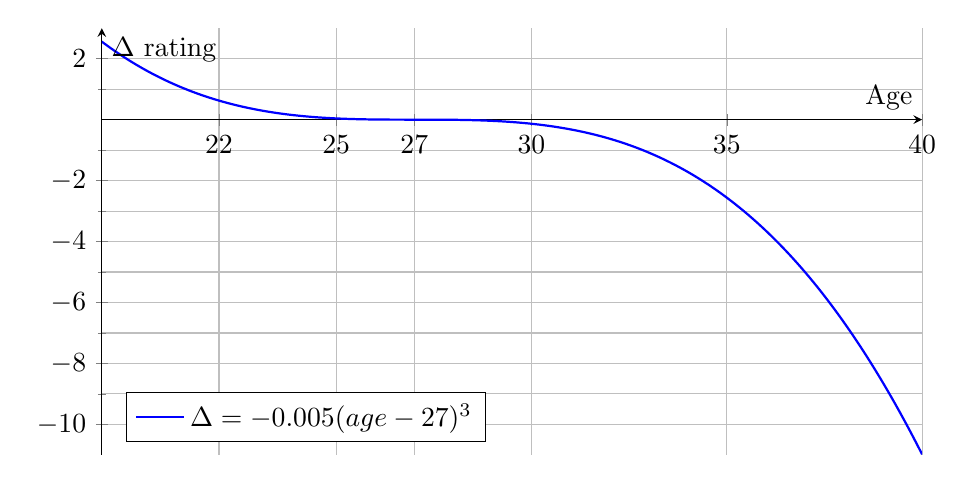
\begin{tikzpicture}
\begin{axis}[
    width=12cm,
    height=7cm,
    xmin=19, xmax=40,
    ymin=-11, ymax=3,
    domain=19:40,
    samples=300,
    axis lines=middle,
    xlabel={Age},
    ylabel={$\Delta$ rating},
    xtick={19,22,25,27,30,35,40},
    ytick={-10,-8,-6,-4,-2,0,2},
    grid=both,
    minor tick num=1,
    legend pos=south west,
]
\addplot[thick, blue]
{-0.005*(x-27)^3};
\addlegendentry{$\Delta=-0.005(age-27)^3$}
\end{axis}
\end{tikzpicture}
\caption{Expected change in player rating as a function of age.}
\label{fig:evolution_curve}
\end{figure}

The function I use is:

\begin{equation}
    \delta = -0.005 * (\text{age} - 27) ** 3 + \epsilon
\end{equation}

Where $\epsilon$ is some noise. For now I hardcode it as $\epsilon = 0.5$, but I have also considered making it a function of the rating (so really good players decline more, or improve faster, but I am not sure about that yet.) 

\paragraph{RL training} I am also happy to announce that I was able to make an RLlib model train on this environment for the very first time! It was a bit of a pain to get it to work because of dependencies and missing packages (turns out RLlib isn't all that great in Windows) but it trained in the end, which I am happy about.

For the rewards, I used this exponential decay function, with $k = 0.3$:

\begin{equation}
    r = e ^ {-k (\text{position} - 1)} 
\end{equation}

\begin{figure}[htbp]
\centering
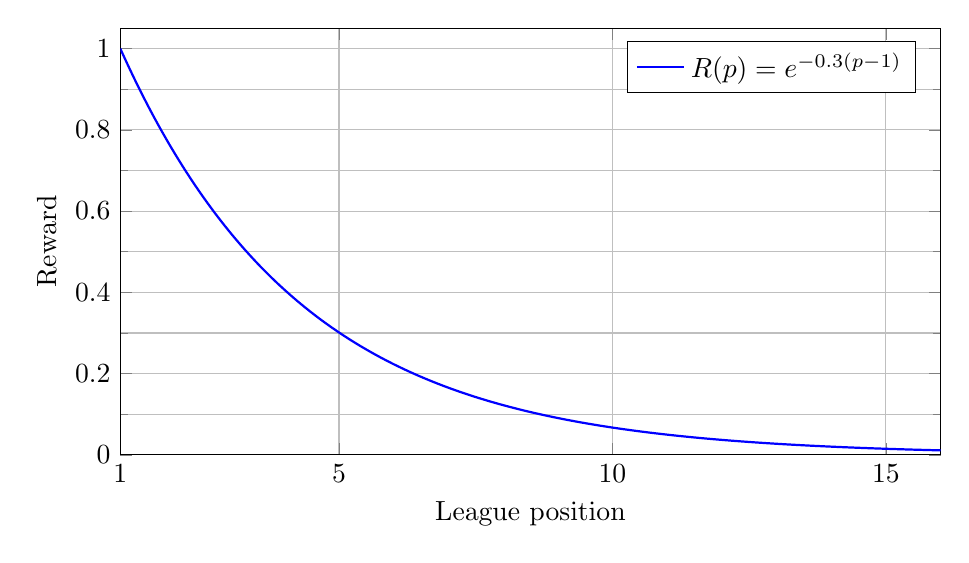
\begin{tikzpicture}
\begin{axis}[
    width=12cm,
    height=7cm,
    xmin=1, xmax=16,
    ymin=0, ymax=1.05,
    domain=1:20,
    samples=300,
    xlabel={League position},
    ylabel={Reward},
    xtick={1,5,10,15,20},
    ytick={0,0.2,0.4,0.6,0.8,1.0},
    grid=both,
    minor tick num=1,
    legend pos=north east,
]

\addplot[
    thick,
    blue,
]
{exp(-0.3*(x-1))};

\addlegendentry{$R(p)=e^{-0.3(p-1)}$}

\end{axis}
\end{tikzpicture}
\caption{Reward curve for teams in positions 1-16}
\end{figure}

The function applies to all teams in playoff positions (1-16, for now). Teams that did not make it also get the same reward function, but first they go through the draft lottery (with the current ruleset), and are assigned rewards based on that. So basically, they can have just as high rewards, but it is uncertain in which position they will land.

I will now work on player retirement and adding new players through some sort of draft or bidding process.



\subsection{\date{June 20, 2026}}

Currently, I have managed to build a small simulation of basketball season games. It is an exceedingly simple simulation, but one that provides a strong basis for future work and small RL experiments. Important features are the following:

\paragraph{Player Attributes}
Players are defined by a single number, which for now I call their \textbf{impact} score. I drew from a lognormal distribution with parameters $\mu = 0$ and $\sigma = 1$. I played around with a pareto/power-law distribution as well, but that seemed too extreme for my taste. There were many not-so-great players and some which had absolutely run-away scores. The lognormal has the heavy-tailed aspect but it isn't as extreme as a Pareto distribution. Usually the best player in any given draw is 10 to 15 times better than the average player, which already seems like plenty to me. A pareto distribution usually creates even bigger talent discrepancies.

\paragraph{Talent Distribution}
Currently, players are simply generated by drawing from my prized lognormal distribution and they are randomly allocated to teams. Obviously, this is \textbf{unrealistic}, as talented players may have a preference for playing together (playing for winners) or for teams with capspace --- something I will have to figure out how to implement. For now teams cannot trade or sign players. I expect that already when this functionality is implemented that talent will eventually be distributed in a more realistic way.

\paragraph{Game Simulation}
Currently games are simulated in a very simple manner. A team has 10 players assigned to it, each with their skill score, which I will refer to as $s_p$ as the score of player p. The sum of the scores of all players in the team $i$ will generate $S_i$, the total score for team $i$:

\begin{equation}
    S_i = \sum_{p \in i} s_p
\end{equation}

($p \in i$) indicates that player $p$ plays for team $i$.

Games are decided by:
\begin{equation}
    P(\text{Team } i \text{ wins}) = S_i - S_j + \epsilon
\end{equation}

Where $\epsilon \sim \text{Logistic}(0, \sigma_{\text{noise}})$. If $S_i - S_j + \epsilon > 0$, team $i$ is assigned as the winner of the game. 

There are many problems with this approach. First, the best player and the end-of-the-bench player all have equal contribution under this scheme, whereas in the NBA it is unlikely the 10th best player would see much gametime. I need to devise a scheme where players get more gametime according to their skill or --- which would be even better --- I allow my RL model to devise a rotation under some contraints (no player can play more than 48 minutes; 240 minutes have to be apportioned in total). I might have to implement an injury or fatigue related mechanism for that if I want to prevent agents from abusing their best player, or I keep their minutes artificially below a certain threshold (40 minutes, for example).

Second, players cannot be described by a single skill score. In reality we have players that can shoot, players that can pass, those that defend the perimeter, some that defend the paint, slashers, post-up players, mid-range specialists and so on. While it would be lovely to be able to simulate games with that level of granularity, the focus of the project is more on the behaviour of basketball teams, especially as it pertains to tanking. For now, I will forego these complicated simulations (also in the interest of time) and go ahead with my singular impact score. As the project develops I will also consider breaking this down into offensive ability score and defensive ability score, $s_{\text{off}}$ and $s_{\text{def}}$.

Building on from the last point, for now I simply draw players from this lognormal distribution, whose parameters I decided on. In a dream scenario, I would be able to use a latent-factor modelling approach to calibrate this distribution for players. That would make this much more interesting and realistic. Otherwise I could also try to incorporate some ready-made impact metrics like PIPM, xRAPM, LEBRON, and DARKO. Or a statistical model of basketball games, but that seems to take me away from the point of the project already.

Third, and for now last, is the logistic noise that I use, with variance $\sigma_{\text{noise}}$. This is very important in calibrating the share of matches that are decided by pure skill versus the natural variance in luck. 

I simulated 16 seasons while respecting the NBA's scheduling style (more games within a division and conference), and I guesstimated some of the parameters. The win percentage I get with my simulation method is actually decently good for being so simple. Look at the plot below, where I compare the win pct distributions I get in simulation with the actual distribution of win percentages from the 2010-11 season.

\begin{figure}
    \centering
    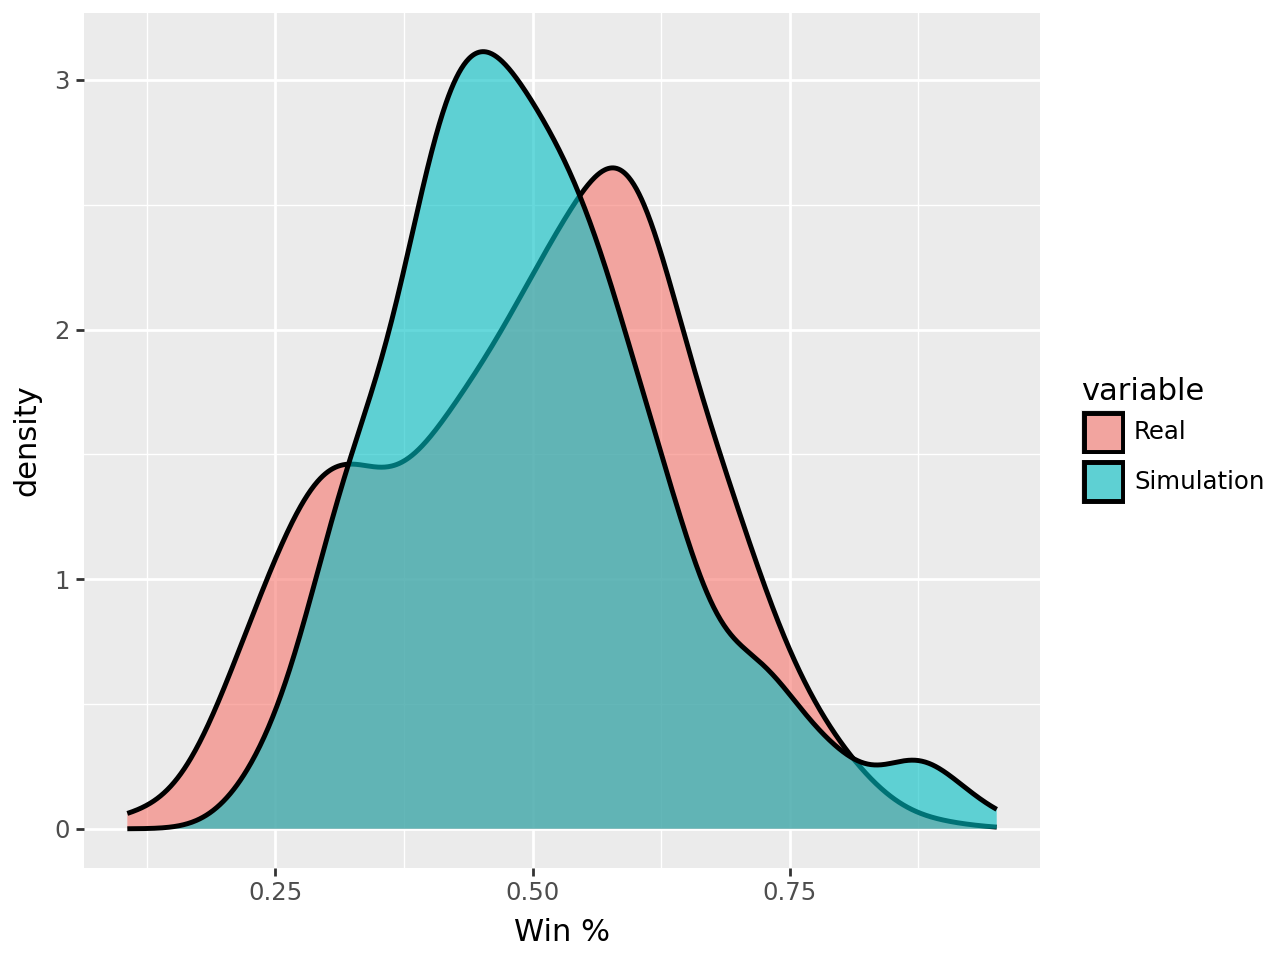
\includegraphics[width=0.75\textwidth]{figs/win_pct_plot.png}
    \caption{First look at simulated vs real win percentage. I don't get the slightly bimodal distribution yet, but I hope this will happen once teams start to make choices.}
\end{figure}


% \section{Reading List}
% \cite{goktasInfiniteHorizonMarkov2025}

% \section{Bibliography}
% \printbibliography


\end{document}